\chapter{Proverb 6}

\begin{figure}
  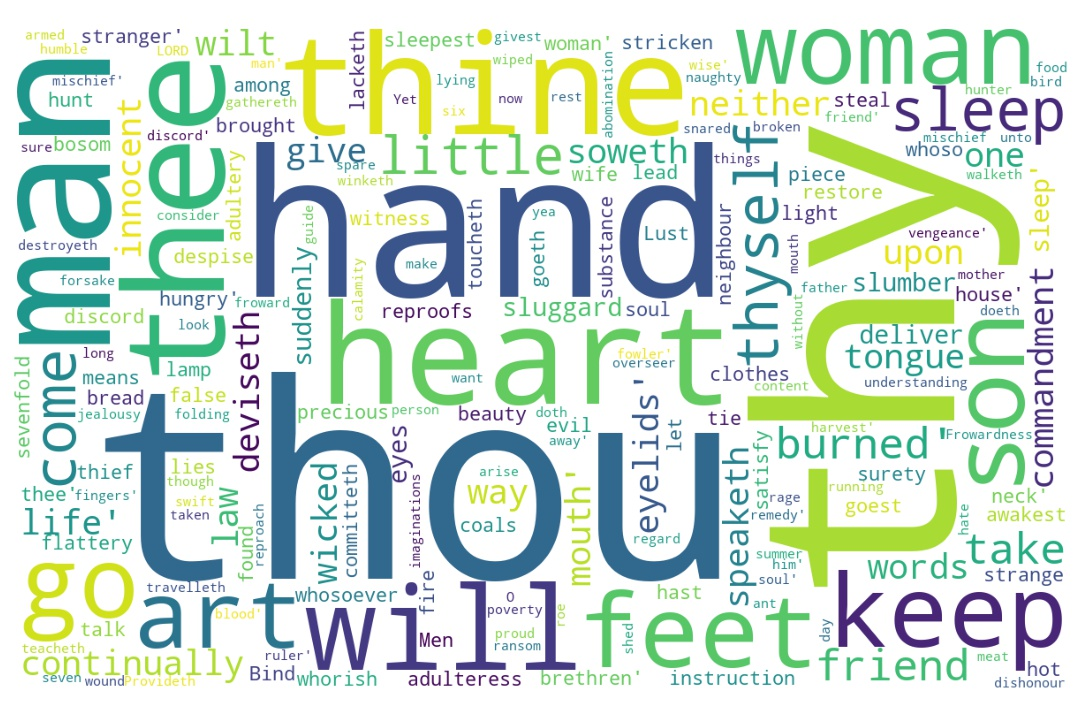
\includegraphics[width=\linewidth]{20OT-Proverbs/Proverb6-WordCloud.jpg}
  \caption{Proverb 6 Word Cloud}
  \label{fig:Proverb 6 Word Cloud}
\end{figure}

\marginpar{\scriptsize \centering \fcolorbox{bone}{lime}{\textbf{THINGS NOT TO DO}}\\ (Proverb 6:1-5) \begin{compactenum}[I.][8]
    \item \textbf{Don't Become Liable} \index[scripture]{Proverbs!Pro 06:01-03}(Proverbs 6:1-3) - and when you do, get out of that liability
    \item \textbf{Don't Became Lazy} \index[scripture]{Proverbs!Pro 06:04}(Pro 6:4) 
    \item \textbf{Don't Lie} \index[scripture]{Proverbs!Pro 06:12, 19} (Pro 6:12, 19) 
    \item \textbf{Don't get an Evil Longing}  \index[scripture]{Proverbs!Pro 06:14}(Pro 6:14) 
    \item \textbf{Don't Get a Proud Look} \index[scripture]{Proverbs!Pro 06:17}(Pro 6:17)
    \item \textbf{Don't Yield to Lust} \index[scripture]{Proverbs!Pro 06:25}(Pro 6:25)
    \item \textbf{Don't Lack Understanding} \index[scripture]{Proverbs!Pro 06:32}(Pro 6:32)
\end{compactenum}}

\footnote{\textcolor[cmyk]{0.99998,1,0,0}{\hyperlink{TOC}{Return to end of Table of Contents.}}}\footnote{\href{https://www.audioverse.org/english/audiobibles/books/ENGKJV/O/Prov/1}{\textcolor[cmyk]{0.99998,1,0,0}{Proverbs Audio}}}\textcolor[cmyk]{0.99998,1,0,0}{My son, if thou be \fcolorbox{bone}{lime}{surety} for thy friend, \emph{if} thou hast stricken thy hand with a stranger,}\
[2] \textcolor[cmyk]{0.99998,1,0,0}{Thou art snared with the words of thy mouth, thou art taken with the words of thy mouth.}\
[3] \textcolor[cmyk]{0.99998,1,0,0}{Do this now, my son, and deliver thyself, when thou art come into the hand of thy friend; go, humble thyself, and make sure thy friend.}
[4] \textcolor[cmyk]{0.99998,1,0,0}{Give not sleep to thine eyes, nor \fcolorbox{bone}{lime}{slumber} to thine eyelids.}
[5] \textcolor[cmyk]{0.99998,1,0,0}{Deliver thyself as a roe from the hand \emph{of} \emph{the} \emph{hunter}, and as a bird from the hand of the fowler.}
[6] \textcolor[cmyk]{0.99998,1,0,0}{Go to the ant, thou sluggard; consider her ways, and be wise:}
[7] \textcolor[cmyk]{0.99998,1,0,0}{Which having no guide, overseer, or ruler,}
[8] \textcolor[cmyk]{0.99998,1,0,0}{Provideth her meat in the summer, \emph{and} gathereth her food in the harvest.}
[9] \textcolor[cmyk]{0.99998,1,0,0}{How long wilt thou sleep, O sluggard? when wilt thou arise out of thy sleep?}
[10] \textcolor[cmyk]{0.99998,1,0,0}{\emph{Yet} a little sleep, a little slumber, a little folding of the hands to sleep:}
[11] \textcolor[cmyk]{0.99998,1,0,0}{So shall thy poverty come as one that travelleth, and thy want as an armed man.}
[12] \textcolor[cmyk]{0.99998,1,0,0}{A naughty person, a wicked man, walketh with a \fcolorbox{bone}{lime}{froward} mouth.}
[13] \textcolor[cmyk]{0.99998,1,0,0}{He winketh with \fcolorbox{bone}{bone}{his} eyes, he speaketh with \fcolorbox{bone}{bone}{his} feet, he teacheth with \fcolorbox{bone}{bone}{his} fingers;}
[14] \textcolor[cmyk]{0.99998,1,0,0}{Frowardness \emph{is} \fcolorbox{bone}{lime}{in \fcolorbox{bone}{bone}{his} heart}, he deviseth mischief continually; he soweth discord.}
[15] \textcolor[cmyk]{0.99998,1,0,0}{Therefore shall \fcolorbox{bone}{bone}{his} calamity come suddenly; suddenly shall he be broken without remedy.}
[16] \textcolor[cmyk]{0.99998,1,0,0}{These six \emph{things} doth the LORD hate: yea, seven \emph{are} an abomination unto him:} %\marginpar{\scriptsize %\textcolor[rgb]{0.00,0.545,0.269}{$\rightarrow$7 Abominations: 
%\begin{compactenum}
%	\item A proud look,
%	\item a lying tongue,
%	\item hands that shed innocent blood,
%	\item An heart that deviseth wicked imaginations,
%	\item feet that be swift in running to mischief,
%	\item A false witness that speaketh lies, and
%	\item he that soweth discord among brethren.
%\end{compactenum}}}
[17] \textcolor[cmyk]{0.99998,1,0,0}{A \fcolorbox{bone}{lime}{proud look}, a lying tongue, and hands that shed innocent blood,}
[18] \textcolor[cmyk]{0.99998,1,0,0}{An heart that deviseth wicked imaginations, feet that be swift in running to mischief,}
[19] \textcolor[cmyk]{0.99998,1,0,0}{A false witness \emph{that} speaketh lies, and he that soweth discord among brethren.}
[20] \textcolor[cmyk]{0.99998,1,0,0}{My son, keep thy father's commandment, and forsake not the law of thy mother:}
[21] \textcolor[cmyk]{0.99998,1,0,0}{Bind them continually upon thine heart, \emph{and} tie them about thy neck.}
[22] \textcolor[cmyk]{0.99998,1,0,0}{When thou goest, it shall lead thee; when thou sleepest, it shall keep thee; and \emph{when} thou awakest, it shall talk with thee.}
[23] \textcolor[cmyk]{0.99998,1,0,0}{For the commandment \emph{is} a lamp; and the law \emph{is} light; and reproofs of instruction \emph{are} the way of life:}\footnote{\textbf{Psalm 119:105} - Thy word is a lamp unto my feet, and a light unto my path.}
[24] \textcolor[cmyk]{0.99998,1,0,0}{To keep thee from the evil woman, from the flattery of the tongue of a strange woman.}
[25] \textcolor[cmyk]{0.99998,1,0,0}{\fcolorbox{bone}{lime}{Lust not} after her beauty in thine heart; neither let her take thee with her eyelids.}
[26] \textcolor[cmyk]{0.99998,1,0,0}{For by means of a whorish woman \emph{a} \emph{man} \emph{is} \emph{brought} to a piece of bread: and the adulteress will hunt for the precious life.}
[27] \textcolor[cmyk]{0.99998,1,0,0}{Can a man take fire in \fcolorbox{bone}{bone}{his} bosom, and \fcolorbox{bone}{bone}{his} clothes not be burned?}
[28] \textcolor[cmyk]{0.99998,1,0,0}{Can one go upon hot coals, and \fcolorbox{bone}{bone}{his} feet not be burned?}
[29] \textcolor[cmyk]{0.99998,1,0,0}{So he that goeth in to \fcolorbox{bone}{bone}{his} neighbour's wife; whosoever toucheth her shall not be innocent.}\footnote{\textbf{1 Corinthians 7:1} - Now concerning the things whereof ye wrote unto me: It is good for a man not to touch a woman.}
[30] \textcolor[cmyk]{0.99998,1,0,0}{\emph{Men} do not despise a thief, if he steal to satisfy \fcolorbox{bone}{bone}{his} soul when he is hungry;}
[31] \textcolor[cmyk]{0.99998,1,0,0}{But \emph{if} he be found, he shall restore sevenfold; he shall give all the substance of \fcolorbox{bone}{bone}{his} house.}
[32] \textcolor[cmyk]{0.99998,1,0,0}{\emph{But} whoso committeth adultery with a woman \fcolorbox{bone}{lime}{lacketh \fcolorbox{bone}{MYGOLD}{understanding}}: he \emph{that} doeth it destroyeth \fcolorbox{bone}{bone}{his} own soul.}
[33] \textcolor[cmyk]{0.99998,1,0,0}{A wound and dishonour shall he get; and \fcolorbox{bone}{bone}{his} reproach shall not be wiped away.}
[34] \textcolor[cmyk]{0.99998,1,0,0}{For jealousy \emph{is} the rage of a man: therefore he will not spare in the day of vengeance.}
[35] \textcolor[cmyk]{0.99998,1,0,0}{He will not regard any ransom; neither will he rest content, though thou givest many gifts.}





